
\documentclass[letterpaper,hide notes,xcolor={table,svgnames},pdftex,10pt]{beamer}
\def\showexamples{t}


%\usepackage[svgnames]{xcolor}

%% Demo talk
%\documentclass[letterpaper,notes=show]{beamer}

\usecolortheme{crane}
\setbeamertemplate{navigation symbols}{}

\usetheme{MyPittsburgh}
%\usetheme{Frankfurt}

%\usepackage{tipa}

\usepackage{hyperref}
\usepackage{graphicx,xspace}
\usepackage[normalem]{ulem}
\usepackage{multicol}

\newcommand\SF[1]{$\bigstar$\footnote{SF: #1}}

\usepackage[default]{sourcesanspro}
\usepackage[T1]{fontenc}

\newcounter{tmpnumSlide}
\newcounter{tmpnumNote}

% old question code
%\newcommand\question[1]{{$\bigstar$ \small \onlySlide{2}{#1}}}
% \newcommand\nquestion[1]{\ifdefined \presentationonly \textcircled{?} \fi \note{\par{\Large \textbf{?}} #1}}
% \newcommand\nanswer[1]{\note{\par{\Large \textbf{A}} #1}}


 \newcommand\mnote[1]{%
   \addtocounter{tmpnumSlide}{1}
   \ifdefined\showcues {~\tiny\fbox{\arabic{tmpnumSlide}}}\fi
   \note{\setlength{\parskip}{1ex}\addtocounter{tmpnumNote}{1}\textbf{\Large \arabic{tmpnumNote}:} {#1\par}}}

\newcommand\mmnote[1]{\note{\setlength{\parskip}{1ex}#1\par}}

%\newcommand\mnote[2][]{\ifdefined\handoutwithnotes {~\tiny\fbox{#1}}\fi
% \note{\setlength{\parskip}{1ex}\textbf{\Large #1:} #2\par}}

%\newcommand\mnote[2][]{{\tiny\fbox{#1}} \note{\setlength{\parskip}{1ex}\textbf{\Large #1:} #2\par}}

\newcommand\mquestion[2]{{~\color{red}\fbox{?}}\note{\setlength{\parskip}{1ex}\par{\Large \textbf{?}} #1} \note{\setlength{\parskip}{1ex}\par{\Large \textbf{A}} #2\par}\ifdefined \presentationonly \pause \fi}

\newcommand\blackboard[1]{%
\ifdefined   \showblackboard
  {#1}
  \else {\begin{center} \fbox{\colorbox{blue!30}{%
         \begin{minipage}{.95\linewidth}%
           \hspace{\stretch{1}} Some space intentionally left blank; done at the blackboard.%
         \end{minipage}}}\end{center}}%
         \fi%
}



%\newcommand\q{\tikz \node[thick,color=black,shape=circle]{?};}
%\newcommand\q{\ifdefined \presentationonly \textcircled{?} \fi}

\usepackage{listings}
\lstset{%
  keywordstyle=\bfseries,
  aboveskip=15pt,
  belowskip=15pt,
  captionpos=b,
  identifierstyle=\ttfamily,
  escapeinside={(*@}{@*)},
  stringstyle=\ttfamiliy,
  frame=lines,
  numbers=left, basicstyle=\scriptsize, numberstyle=\tiny, stepnumber=0, numbersep=2pt}

\usepackage{siunitx}
\newcommand\sius[1]{\num[group-separator = {,}]{#1}\si{\micro\second}}
\newcommand\sims[1]{\num[group-separator = {,}]{#1}\si{\milli\second}}
\newcommand\sins[1]{\num[group-separator = {,}]{#1}\si{\nano\second}}
\sisetup{group-separator = {,}, group-digits = true}

%% -------------------- tikz --------------------
\usepackage{tikz}
\usetikzlibrary{positioning}
\usetikzlibrary{arrows,backgrounds,automata,decorations.shapes,decorations.pathmorphing,decorations.markings,decorations.text}

\tikzstyle{place}=[circle,draw=blue!50,fill=blue!20,thick, inner sep=0pt,minimum size=6mm]
\tikzstyle{transition}=[rectangle,draw=black!50,fill=black!20,thick, inner sep=0pt,minimum size=4mm]

\tikzstyle{block}=[rectangle,draw=black, thick, inner sep=5pt]
\tikzstyle{bullet}=[circle,draw=black, fill=black, thin, inner sep=2pt]

\tikzstyle{pre}=[<-,shorten <=1pt,>=stealth',semithick]
\tikzstyle{post}=[->,shorten >=1pt,>=stealth',semithick]
\tikzstyle{bi}=[<->,shorten >=1pt,shorten <=1pt, >=stealth',semithick]

\tikzstyle{mut}=[-,>=stealth',semithick]

\tikzstyle{treereset}=[dashed,->, shorten >=1pt,>=stealth',thin]

\usepackage{ifmtarg}
\usepackage{xifthen}
\makeatletter
% new counter to now which frame it is within the sequence
\newcounter{multiframecounter}
% initialize buffer for previously used frame title
\gdef\lastframetitle{\textit{undefined}}
% new environment for a multi-frame
\newenvironment{multiframe}[1][]{%
\ifthenelse{\isempty{#1}}{%
% if no frame title was set via optional parameter,
% only increase sequence counter by 1
\addtocounter{multiframecounter}{1}%
}{%
% new frame title has been provided, thus
% reset sequence counter to 1 and buffer frame title for later use
\setcounter{multiframecounter}{1}%
\gdef\lastframetitle{#1}%
}%
% start conventional frame environment and
% automatically set frame title followed by sequence counter
\begin{frame}%
\frametitle{\lastframetitle~{\normalfont(\arabic{multiframecounter})}}%
}{%
\end{frame}%
}
\makeatother

\makeatletter
\newdimen\tu@tmpa%
\newdimen\ydiffl%
\newdimen\xdiffl%
\newcommand\ydiff[2]{%
    \coordinate (tmpnamea) at (#1);%
    \coordinate (tmpnameb) at (#2);%
    \pgfextracty{\tu@tmpa}{\pgfpointanchor{tmpnamea}{center}}%
    \pgfextracty{\ydiffl}{\pgfpointanchor{tmpnameb}{center}}%
    \advance\ydiffl by -\tu@tmpa%
}
\newcommand\xdiff[2]{%
    \coordinate (tmpnamea) at (#1);%
    \coordinate (tmpnameb) at (#2);%
    \pgfextractx{\tu@tmpa}{\pgfpointanchor{tmpnamea}{center}}%
    \pgfextractx{\xdiffl}{\pgfpointanchor{tmpnameb}{center}}%
    \advance\xdiffl by -\tu@tmpa%
}
\makeatother
\newcommand{\copyrightbox}[3][r]{%
\begin{tikzpicture}%
\node[inner sep=0pt,minimum size=2em](ciimage){#2};
\usefont{OT1}{phv}{n}{n}\fontsize{4}{4}\selectfont
\ydiff{ciimage.south}{ciimage.north}
\xdiff{ciimage.west}{ciimage.east}
\ifthenelse{\equal{#1}{r}}{%
\node[inner sep=0pt,right=1ex of ciimage.south east,anchor=north west,rotate=90]%
{\raggedleft\color{black!50}\parbox{\the\ydiffl}{\raggedright{}#3}};%
}{%
\ifthenelse{\equal{#1}{l}}{%
\node[inner sep=0pt,right=1ex of ciimage.south west,anchor=south west,rotate=90]%
{\raggedleft\color{black!50}\parbox{\the\ydiffl}{\raggedright{}#3}};%
}{%
\node[inner sep=0pt,below=1ex of ciimage.south west,anchor=north west]%
{\raggedleft\color{black!50}\parbox{\the\xdiffl}{\raggedright{}#3}};%
}
}
\end{tikzpicture}
}


%% --------------------

%\usepackage[excludeor]{everyhook}
%\PushPreHook{par}{\setbox0=\lastbox\llap{MUH}}\box0}

%\vspace*{\stretch{1}

%\setbox0=\lastbox \llap{\textbullet\enskip}\box0}

\setlength{\parskip}{\fill}

\newcommand\noskips{\setlength{\parskip}{1ex}}
\newcommand\doskips{\setlength{\parskip}{\fill}}

\newcommand\xx{\par\vspace*{\stretch{1}}\par}
\newcommand\xxs{\par\vspace*{2ex}\par}
\newcommand\tuple[1]{\langle #1 \rangle}
\newcommand\code[1]{{\sf \footnotesize #1}}
\newcommand\ex[1]{\uline{Example:} \ifdefined \presentationonly \pause \fi
  \ifdefined\showexamples#1\xspace\else{\uline{\hspace*{2cm}}}\fi}

\newcommand\ceil[1]{\lceil #1 \rceil}


\AtBeginSection[]
{
   \begin{frame}
       \frametitle{Outline}
       \tableofcontents[currentsection]
   \end{frame}
}



\pgfdeclarelayer{edgelayer}
\pgfdeclarelayer{nodelayer}
\pgfsetlayers{edgelayer,nodelayer,main}

\tikzstyle{none}=[inner sep=0pt]
\tikzstyle{rn}=[circle,fill=Red,draw=Black,line width=0.8 pt]
\tikzstyle{gn}=[circle,fill=Lime,draw=Black,line width=0.8 pt]
\tikzstyle{yn}=[circle,fill=Yellow,draw=Black,line width=0.8 pt]
\tikzstyle{empty}=[circle,fill=White,draw=Black]
\tikzstyle{bw} = [rectangle, draw, fill=blue!20, 
    text width=4em, text centered, rounded corners, minimum height=2em]
    
    \newcommand{\CcNote}[1]{% longname
	This work is licensed under the \textit{Creative Commons #1 3.0 License}.%
}
\newcommand{\CcImageBy}[1]{%
	\includegraphics[scale=#1]{creative_commons/cc_by_30.pdf}%
}
\newcommand{\CcImageSa}[1]{%
	\includegraphics[scale=#1]{creative_commons/cc_sa_30.pdf}%
}
\newcommand{\CcImageNc}[1]{%
	\includegraphics[scale=#1]{creative_commons/cc_nc_30.pdf}%
}
\newcommand{\CcGroupBySa}[2]{% zoom, gap
	\CcImageBy{#1}\hspace*{#2}\CcImageNc{#1}\hspace*{#2}\CcImageSa{#1}%
}
\newcommand{\CcLongnameByNcSa}{Attribution-NonCommercial-ShareAlike}

\newenvironment{changemargin}[1]{% 
  \begin{list}{}{% 
    \setlength{\topsep}{0pt}% 
    \setlength{\leftmargin}{#1}% 
    \setlength{\rightmargin}{1em}
    \setlength{\listparindent}{\parindent}% 
    \setlength{\itemindent}{\parindent}% 
    \setlength{\parsep}{\parskip}% 
  }% 
  \item[]}{\end{list}} 




\title{Lecture 32 --- Ethics: A Psychological Basis }

\author{Jeff Zarnett, based on original by Douglas Harder \\ \small \texttt{jzarnett@uwaterloo.ca} / \texttt{dwharder@uwaterloo.ca}}
\institute{Department of Electrical and Computer Engineering \\
  University of Waterloo}
\date{\today}


\begin{document}

\begin{frame}
  \titlepage

\begin{center}
  \small{Acknowledgments: Douglas Harder~\cite{dwh}, Julie Vale~\cite{jv}}
  \end{center}
\end{frame}




\begin{frame}
\frametitle{Ethics and Science}

Ethics used to be entirely in the domain of philosophy.

Today, we have the ability to image the brain and apply neuroscience and other scientific study techniques. 

Ethics is slowly being moving from art to science.

\end{frame}



\begin{frame}
\frametitle{Ethics and Science}

Consider light:
\begin{itemize}
\item Light forms a continuous spectrum of infinitely many colours
\item The human eye is sufficiently sensitive that we require 24-bit colour to represent colours faithfully:  $2^{24} = 16 777 216$ different colours
\item We do not, however, require that many colours -- each colour can be represented by different combinations of three colours
\item It is a three-dimensional space
\end{itemize}


\end{frame}



\begin{frame}
\frametitle{Break Out Your Crayons}

Chances are you learned in school that the primary colours are red, yellow, and blue.

This is ``wrong'' -- it's analogous to picking a non-orthogonal basis is linear algebra:  it's exceptionally inefficient.

(It is, however, excellent for mixing finger paints!)

The additive colour basis can be represented as red-green-blue:

\includegraphics[width=0.1\textwidth]{images/rgb}

A subtractive colour basis is cyan-magenta-yellow:

\includegraphics[width=0.1\textwidth]{images/cmy}

\end{frame}



\begin{frame}
\frametitle{Ethics and Science}

Can we break ethics down into quantifiable items that can be measured?

With functional magnetic resonance imaging (fMRI) we can now begin to probe the human brain.

The human brain -- not surprisingly -- seems to be finite dimensional, as well.

There is still much we do not understand about how the brain works, but research continues.

\end{frame}



\begin{frame}
\frametitle{Probing the Brain}

A part of the brain is associated with counting small numbers.

In the intraparietal sulcus, different neurons will become excited if you view one, two, three, four, or more objects.

Infants respond to changes in stimulation and become uninterested in continuity.

Always showing two of particular items will soon disinterest the infant.

Showing different numbers of thes ame object will keep the infant's attention -- a different part of the brain is activated by the number.


\end{frame}



\begin{frame}
\frametitle{Ethics are Societal and Biological}

Ethics is an evolved trait and depends on:
\begin{itemize}
\item Human societies
\item The characteristics of the human species
\end{itemize}

Examples:

Shaking hands is reasonable, because little or no harm can come of it\\
\quad Normal in Western society; bowing is appropriate in Eastern cultures.

Contact with a stranger's face is unacceptable; too high a risk of damage.\\
\quad It takes trust to allow others to touch the face.

If humans had thicker skin, greater protection around the eyes, such contact might be acceptable/normal.

\end{frame}



\begin{frame}
\frametitle{Ethics and Science}

Drinking and driving is seen as immoral.\\
\quad Drinking alcohol is not immoral (in most societies; not all).\\
\quad Driving a vehicle is not immoral. 

Yet the combination of them is! 


Alcohol adversely affects human performance and that degradation can and will adversely affect others (e.g., car crash).

\end{frame}



\begin{frame}
\frametitle{We are but mortal...}

Killing another human is seen as unacceptable, but there are circumstances in which is it seen as permitted.

You may agree or disagree with some or all of the following examples:

\begin{itemize}
	\item If someone is threatening your life (or the lives of others), it is acceptable to defend oneself even if it means killing the other person.
	\item During a war, it is acceptable to kill the soldiers of the opposing forces.
	\item It is acceptable to execute prisoners convicted of heinous crimes.
	\item Some see killing as an acceptable response to blasphemy or apostasy.
\end{itemize}

\end{frame}



\begin{frame}
\frametitle{The Moral Compass}

Based on examinations of the brain with fMRI technology, scientists posit that humans all have the following basic moral evaluation scales:

\begin{center}
\begin{tabular}{l|l}
	\textbf{Positive} & \textbf{Negative} \\ \hline
	Care & Harm \\
	Fairness & Cheating \\
	Liberty & Oppression \\
	Sanctity & Degradation \\
	Loyalty & Betrayal \\
	Authority & Subversion \\
\end{tabular}
	
\end{center}

\end{frame}



\begin{frame}
\frametitle{The Moral Compass}

One may consider ethics as the interconnections between these values.

\begin{center}
	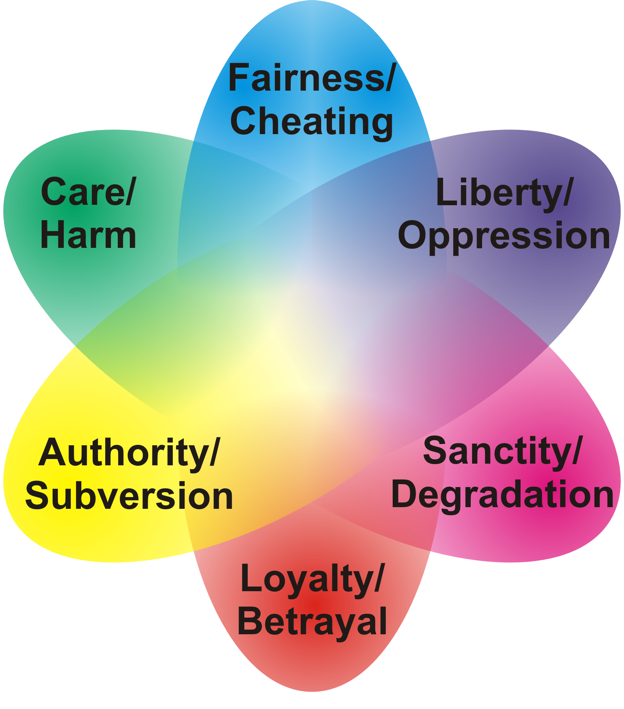
\includegraphics[width=0.5\textwidth]{images/moralcompass}
\end{center}


\end{frame}



\begin{frame}
\frametitle{Nepotism}

Consider nepotism -- the idea of giving favour to one's relatives -- comes from the Italian word for nephew (hiring practices back then were not like now).

Values supporting it: care and loyalty to the family.

In some countries it would be a serious betrayal not to hire your relatives.

The head of government of Trinidad and Tobago recently took her niece on a world-wide
tour, charging her niece's expenses to the country.

\end{frame}



\begin{frame}
\frametitle{Nepotism}

Canadian society, however, frowns upon nepotism.

Everyone else is affected by it: the company, the employees of the company, and ultimately the country as a whole.

Values of fairness to others and preventing harm to others/society are seen as more important than looking after family members.

There are rarely objective answers to such questions...

\end{frame}



\begin{frame}
\frametitle{Five Whys}

All of these values have evolutionary advantage.

This does not, however, mean that each of them is a value that supports civilization and human progress.

Nor does it mean that all values are equally important.


\begin{center}
	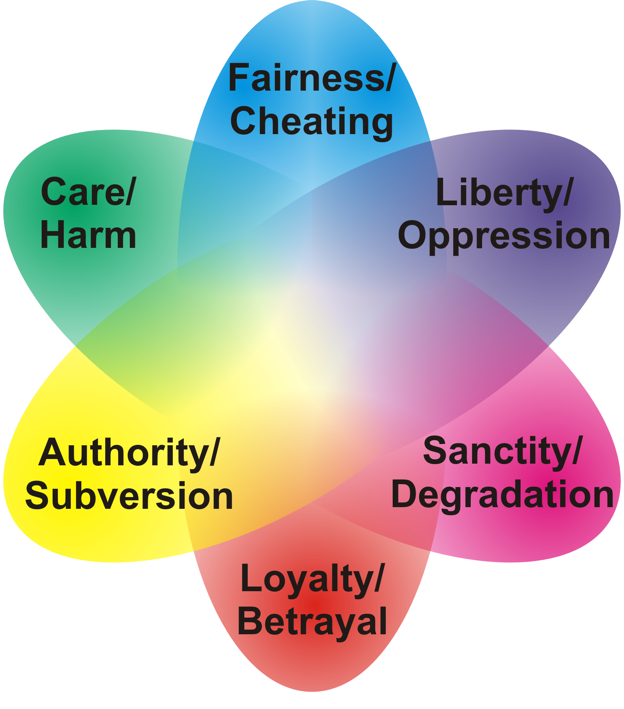
\includegraphics[width=0.2\textwidth]{images/moralcompass}
\end{center}


As an engineer, when you consider any ethical situation, you must consider your choices and why you are taking those choices.
\end{frame}



\begin{frame}
\frametitle{Empathy}

Primates, including humans, have empathy for others in their species.

Mirror neurons will fire when certain activities occur either to oneself or while one is watching someone else.

Sociopathy is associated with an inability to feel empathy.

Narcissism is an abnormal focus on oneself.

\end{frame}



\begin{frame}
\frametitle{Empathy}

Empathy is something that develops as an infant grows into an adult. 

Empathy will be enabled when watching other people in situations involving pain, disgust, or contact.

Most of you will feel pain when others do.\\
\quad How would you feel if your best friend were injured in a car crash?

Consider a picture of a Dalit, covered in excrement, coming up from having cleared a blockage in the sewers of an Indian city.

\end{frame}



\begin{frame}
\frametitle{Sympathy vs Empathy}

There is a distinction between sympathy and empathy, even though the words are sometimes incorrectly used interchangeably. 

Sympathy is acknowledgment of another person's suffering and providing comfort/assistance.

Empathy is understanding how others are feeling (and may be from personal experience or imagining oneself in the other person's place).


\end{frame}



\begin{frame}
\frametitle{Kissing}

Consider two lovers kissing...

\begin{itemize}
\item What if one is a Conservative and the other a Liberal?
\item What if one is a farmer and the other is a movie star?
\item One is a Christian and the other a Muslim?
\item What if one is a Dalit and the other is a Brahmin?
\item What if one is European and the other African?
\item What if they are both men?
\item What if one is 35 years old and the other 13 years old?
\end{itemize}

In some societies such a public display of affection is not acceptable at all.

\end{frame}



\begin{frame}
\frametitle{Liberals vs. Conservatives}

For all the fighting we see in politics about liberals vs. conservatives, both groups have morals and attempt to have them enshrined in society.

The major difference is what morals the sides consider important. 

We will draw a distinction here between small-l liberal and the Liberal Party; equally a distinction between small-c conservative and the Conservative Party.

Just because the party calls itself something does not mean it follows those values, nor do such parties necessarily take the same stances on all issues...

\end{frame}



\begin{frame}
\frametitle{A Question of Values}

Traditional liberal values include care, fairness, liberty...

Traditional libertarian values put a greater emphasis on liberty:\\
\quad Freedom, individual liberty, voluntary association...

Traditional conservative values include authority, loyalty, sanctity (that generally liberal values de-emphasize).

Fascist values put even more emphasis on authority and loyalty.

\end{frame}



\begin{frame}
\frametitle{You Gotta Fight...}

When you are attacked physically, your brain responds by entering into a defensive state which essentially bypasses the higher functioning of the brain.


With the evolution of reasoning, your brain will respond in a similar manner if your ideas are attacked.

\end{frame}



\begin{frame}
\frametitle{Cleanliness}

It is necessary for any species to avoid harmful objects -- e.g., rotten fruit and meat
Keeping clean, eating healthy food, etc., is beneficial. 

Consequently, we will have averse reactions to un-cleanliness.

One consequence manifestation of this is in the cleanliness of the body -- both inside and out.

Consider drug use...

\end{frame}



\begin{frame}
\frametitle{What are you, a spy or something?!}


You may notice the strong revulsion against spies -- even those from the other side who help us.


Again, countries have co-opted and transferred what used to be a loyalty to the tribe to a geo-political organization.

More important than anything else are the invisible lines we have chosen to partition this world into...?

Sometimes... sometimes it's about culture more than the nation... many countries would gladly take some land off their neighbours' hands...
\end{frame}



\begin{frame}
\frametitle{ME GOOD THEM BAD}

When you reach a different ethical conclusion from someone else, it's not that they're immoral -- they simply have different values.

The United States Congress has an interesting aspects.

The outside polarization of Republican -- Democrat appears very strong when compared to the Canadian multi-party system.

There are, however, many more bi-partisan communication and significantly fewer restrictions w.r.t. voting along party lines.

In Canada, voting along party lines is considered much more essential due to non-confidence votes.


\end{frame}



\begin{frame}
\frametitle{Ethics and Professional Misconduct}

There is an official PEO Code of Ethics.

We will now examine it, and the definition of professional misconduct, in the light of the value compass:

\begin{center}
	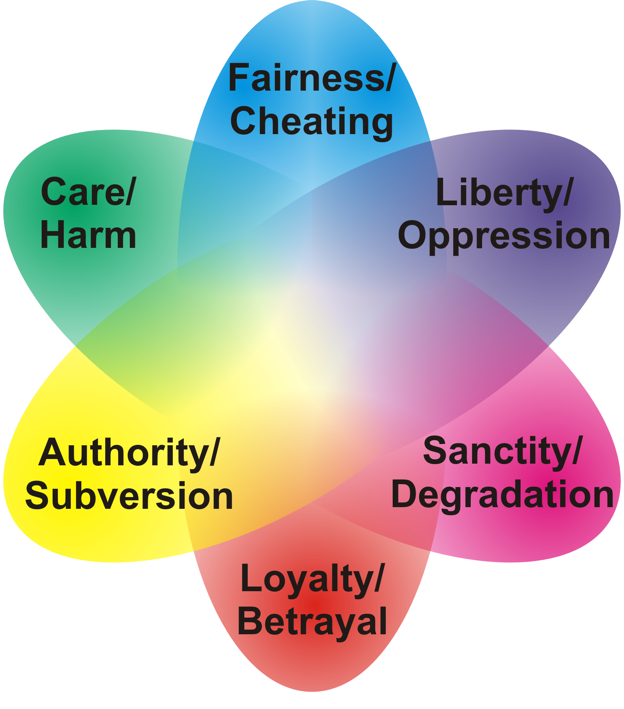
\includegraphics[width=0.4\textwidth]{images/moralcompass}
\end{center}


\end{frame}


\begin{frame}
\frametitle{References \& Disclaimer}
\bibliographystyle{alphaurl}
\setbeamertemplate{bibliography item}{\insertbiblabel}
{\scriptsize
\bibliography{290}
}
\vfill

{\tiny Disclaimer: the material presented in these lectures slides is intended for use in the course ECE~290 at the University of Waterloo and should not be relied upon as legal advice. Any reliance on these course slides by any party for any other purpose are the responsibility of such parties.  The author(s) accept(s) no responsibility for damages, if any, suffered by any party as a result of decisions made or actions based on these course slides for any other purpose than that for which it was intended.\par}


\end{frame}


\end{document}

